\documentclass{beamer}
\DeclareFontShape{OT1}{cmss}{b}{n}{<->ssub * cmss/bx/n}{} 
\usetheme{Szeged}
\usecolortheme{beaver}
\usepackage{amsmath}
\usepackage{amsfonts}
\usepackage{mathbbol}
\usepackage{xcolor} % before tikz or tkz-euclide if necessary
\usepackage{tikz}
%\usepackage{tkz-euclide} % no need to load TikZ
%\usepackage{tikz-cd}
\usepackage{multirow}
\usepackage{lmodern}
\usepackage{bm}
\usepackage{subcaption}
%\usepackage{subfigure}


\usepackage[
backend=biber,
style=authoryear-icomp,
sortlocale=de_DE,
natbib=true,
url=false, 
doi=true,
eprint=false
]{biblatex}
\addbibresource{../Bibliography/main_ML.bib}
\usetikzlibrary{cd}


\titlegraphic{
\includegraphics[width=2cm]{../Figures/UAMS_RGB.png}
}


\title{Bone Journal Club\\ Math Modeling for Bone-Cell Dynamics}
\author{Horacio G\'omez-Acevedo\\ Department of Biomedical Informatics\\
	University of Arkansas for Medical Sciences}

\begin{document}
	\begin{frame}[plain]
		\maketitle
	\end{frame}

\begin{frame}{Overview}
	\tableofcontents
\end{frame}

\section{Math Modeling why?}
\begin{frame}{Why?}

\begin{itemize}
	\item It is an attempt to introduce theoretical foundations to biological processes.
	\item It can also explain also some of the paradoxical observations.
	\item Based on "mechanistic" assumptions, models can produce useful predictions. 
	\item Once a model is "calibrated", it can accommodate extensions based on new biological findings. 
\end{itemize}	


\end{frame}
\subsection{Basic Ideas}
\begin{frame}{Compartmental Models}
The so-called \textbf{Compartmental Models} try to describe the dynamics of cell interactions among two or more well-characterized cell types.
 Some basic implicit assumptions about cell populations
\begin{itemize}
	\item The evolution of the population is described by rates (i.e., instant changes in population numbers).
	\item Cells are indistinguishable among the same type ($A$ and $B$ below). 
	\item $A$ and $B$ represent abundance of the given type. 
\end{itemize}
\end{frame}
\begin{frame}{Compartmental Models (cont)}
	
\begin{itemize}
\item Cells are entering (some progenitor cell) into the $A$ compartment at a certain rate $\pi_A$.
\item Cells leave the compartment (cell death) at the rate $\mu_A$ and $\mu_B$, respectively.
\item Cells evolve from Type $A$ into Type $B$ at a rate proportional to their abundance at a constant rate $\beta$.
\end{itemize}	

	\begin{figure}[h]
	\centering
	%	\begin{subfigure}{0.4\textwidth}
		%		\centering
		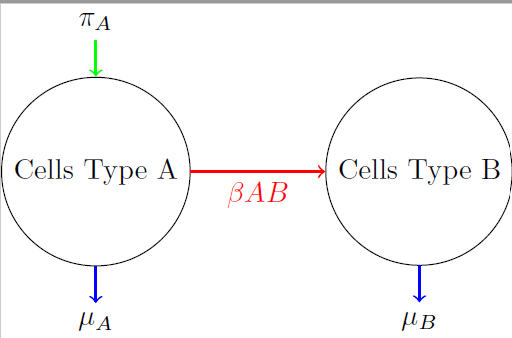
\includegraphics[scale=0.4]{../Figures/fig_compartment.png}
		%	\end{subfigure}
\end{figure}
	
\end{frame}

\begin{frame}{Compartmental Model Math}
The translation of this interaction is translated in the following system of (ordinary) differential equations

\begin{equation}
	\begin{split}
		A'&= \pi_A - \beta A B - \mu_A A \\
		B'&= \beta A B - \mu_B B
	\end{split}
\end{equation}
	\begin{figure}[h]
	\centering
	%	\begin{subfigure}{0.4\textwidth}
		%		\centering
		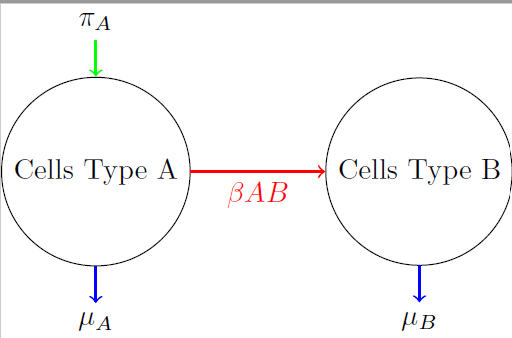
\includegraphics[scale=0.4]{../Figures/fig_compartment.png}
		%	\end{subfigure}
\end{figure}

\end{frame}

\begin{frame}{"Solving" the equations}
	For the above system, we can calculate the "steady state(s)". This means the point(s) that the trajectories will end up reaching (after potentially some very long time) or they are getting away from.
\begin{figure}[h]
	\centering
	%	\begin{subfigure}{0.4\textwidth}
		%		\centering
		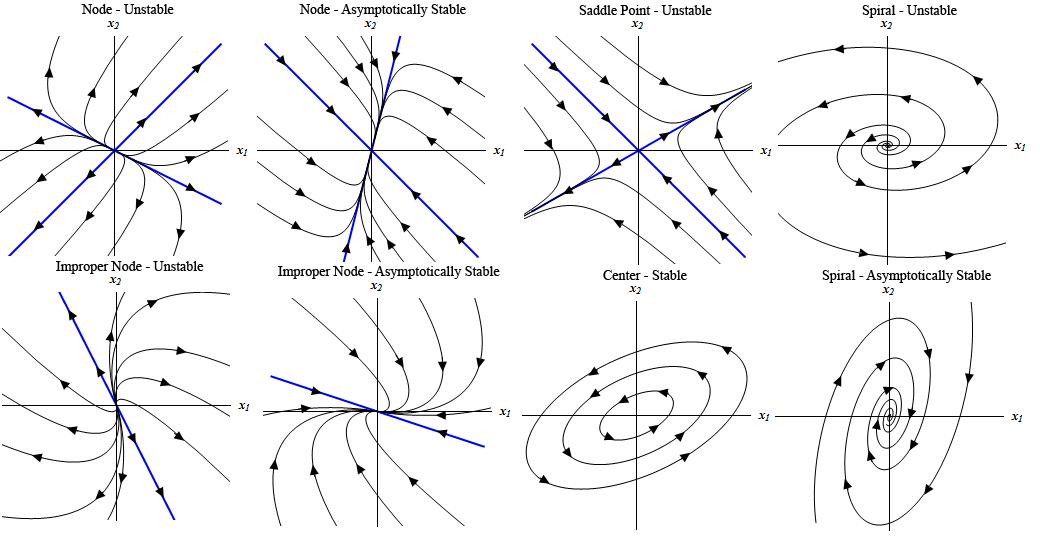
\includegraphics[scale=0.2]{../Figures/fig_dyn_sys.jpg}
		\caption{\href{https://discourse.julialang.org/t/plotting-dynamical-systems-trajectories/46166}{dynamical systems}}
		%	\end{subfigure}
\end{figure}	
	
\end{frame}

\begin{frame}{"Solving" the equations (cont)}
	In general, it is relatively hard to calculate those steady states and determine (locally) their behavior (attractor  or repelor) (\textcolor{red}{Mathematical issue})
	
	Instead, we solve the equations "numerically". Meaning, we write code to simulated the trajectories (e.g., Matlab) for a given set of parameters ($\pi_A$, $\beta$, etc.)
\begin{figure}[h]
	\centering
	%	\begin{subfigure}{0.4\textwidth}
		%		\centering
		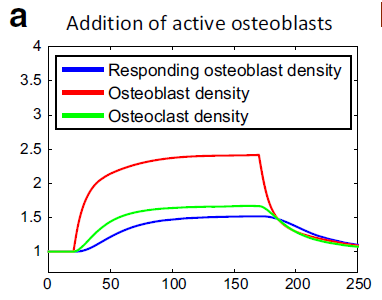
\includegraphics[scale=0.45]{../Figures/fig_numeric_sol.png}
	
		%	\end{subfigure}
\end{figure}		 
	
	
\end{frame}

\begin{frame}{In Silico Simulations}
A great deal of time is spent calculating the parameters from a given established system
\begin{itemize}
	\item Using other literature sources
	\item Making simulations based on newly produced data	
\end{itemize}

The ultimate goal is to produce a tuned \textit{in silico} system based on  equations that mimic fundamental biological concepts. Then, we can explore scenarios and test biological hypothesis. 



\end{frame}


\section{Paper}
\begin{frame}{Today's paper}
	\begin{figure}[h]
		\centering
		%	\begin{subfigure}{0.4\textwidth}
			%		\centering
			
\includegraphics[scale=0.4]{../Figures/lemaire_paper_2019.png}
			%	\end{subfigure}
	\end{figure}
\end{frame}

\subsection{Main Model}
\begin{frame}{Picture First}
		\begin{figure}[h]
		\centering
		%	\begin{subfigure}{0.4\textwidth}
			%		\centering
			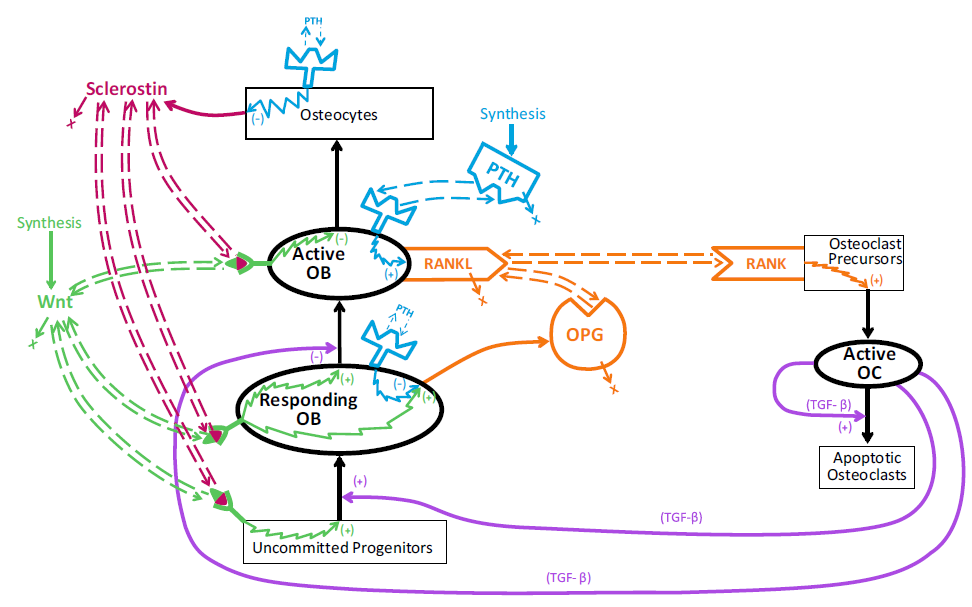
\includegraphics[scale=0.5]{../Figures/fig_lemaire_fig1.png}
			%	\end{subfigure}
	\end{figure}
\end{frame}

\begin{frame}{Cell Compartment Equations}

\begin{equation}
	\begin{split}
	R' &= D_R \pi_C \pi_W - D_B \frac{\pi_W}{\pi_C} R\\
	B' &= D_B \frac{\pi_W}{\pi_C} R - \frac{k_e^B}{\pi_W}B\\
	C' &= D_C \pi_L - k_e^C \pi_C C 
	\end{split}
\end{equation}
According to the model $D_R$, $D_B$ and $D_C$ are constant differentiation rates, $k_e^B$, and $k_e^C$ are constant elimination rates. 

\end{frame}

\subsection{Ligands Competition}
\begin{frame}{Ligands Models}
	The modeling follows the enzymatic theory of Michaelis-Menten.
	In brief, if we have a substrate $S$ reacting with an enzyme $E$ to form a complex $SE$ can be modeled as
\begin{center}
\begin{tikzcd}[ampersand replacement=\&, column sep=small]
	S +E  \arrow[r,shift left, "k_1"] \& S\circ E \arrow[l,shift left,"k_{-1}"]  
\end{tikzcd}
\end{center}	

\begin{equation}
\frac{d S \circ E}{dt}= k_1 S \cdot E - k_{-1} S \circ E
\end{equation}

When the text refers that equations are considered at "steady state" it means that 
\begin{equation*}
	k_1 S \cdot E = k_{-1} S \circ E
\end{equation*}
	
\end{frame}

\begin{frame}{Ligand Models (cont)}
			\begin{figure}[h]
		\centering
		%	\begin{subfigure}{0.4\textwidth}
			%		\centering
			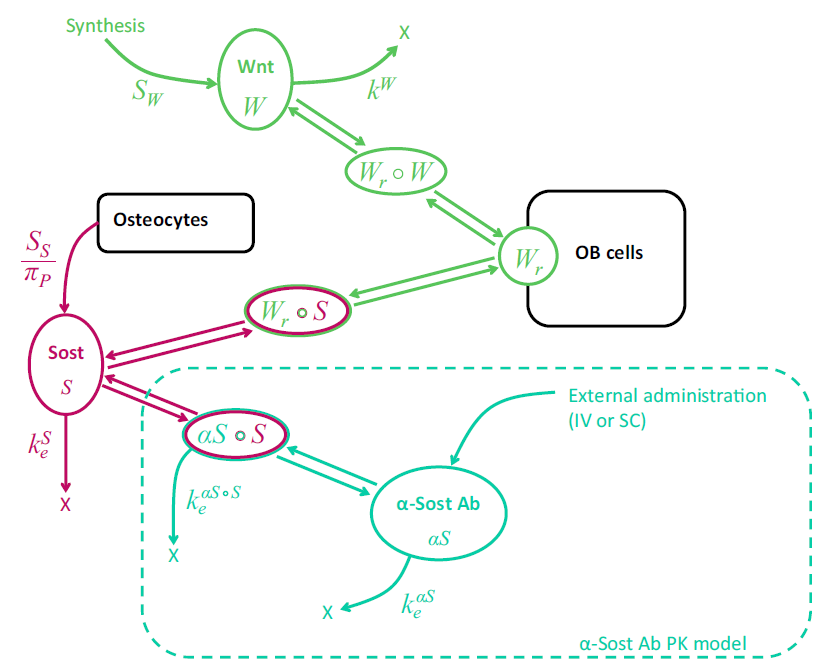
\includegraphics[scale=0.45]{../Figures/fig_lemaire_fig2.png}
			%	\end{subfigure}
	\end{figure}
	
\end{frame}

\begin{frame}{Binding to LPR5/6}
The attachment of Wnt to the receptor $W_r$ is taken at the steady state. 
The equations for binding of Wnt receptor and sclerostin are

\begin{equation}
	\begin{split}
		\frac{d W_r \circ S}{dt} &= k_9 S \cdot W_r - k_{10} W_r \circ S \\
		\frac{d \alpha S  \circ S}{dt} &= k_{13} S \cdot \alpha S - k_{14} \alpha S \circ S -k_e^{\alpha S \circ S} \alpha S \circ S 
	\end{split}
\end{equation}
The second equation represents the presence of an antibody for Sost
\end{frame}

\subsection{Parameters}
\begin{frame}{Parameter Estimation}
\begin{figure}[h]
	\centering
	%	\begin{subfigure}{0.4\textwidth}
		%		\centering
		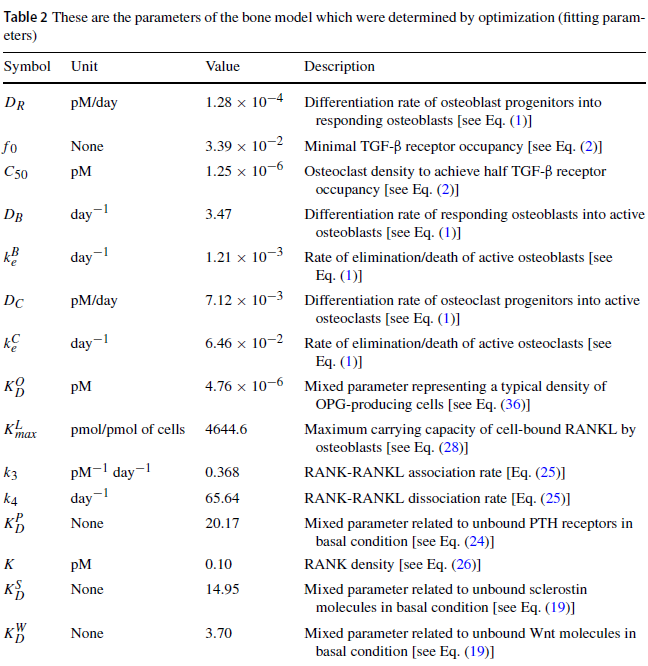
\includegraphics[scale=0.45]{../Figures/fig_lemaire_table2.png}
		%	\end{subfigure}
\end{figure}	
\end{frame}
\subsection{Simulations}

\section{Extensions of the Model}

\subsection{Osteoclast}

\section{Conclusions}

\subsection{What does it take to make the model?}

\subsection{What type of collaboration is necessary?}

\subsection{What type of experiments are required?}

\subsection{Is this the only type of model available?}

	


\begin{frame}{Journal Club Format}
	This is a new format for Journal Club
	\begin{itemize}
		\item We will explore more carefully the methodology.
		\item Most of the papers are going to require "heavy" tools from computer sciences, statistics and mathematics. 
		\item It will be a transition time to understand each other (be patient)
		\item The dynamical nature of brain activity will make it very challenging to hold on to a single model. 
		\item Complexity vs. Explainability is an implicit trade-off. 
		\item The ultimate goal is to use and expand "acceptable" methodologies into new and more "appropriate" ones. Yes, this means \textbf{coding} (R, Python, MatLab).
	\end{itemize} 
\end{frame}

\begin{frame}{Hidden Markov Models}
	The implementation of Hidden Markov models dates back in the late 60's by Leonard Baum and collaborators. It is still an active area of research. 	
	
	What is a Markov chain?
	\begin{figure}[h]
		\centering
		%	\begin{subfigure}{0.4\textwidth}
			%		\centering
			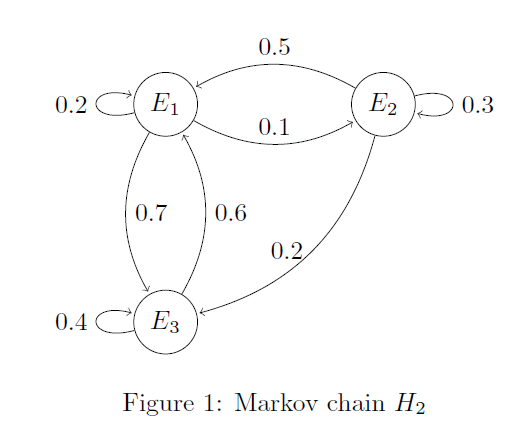
\includegraphics[scale=0.6]{../Figures/fig_markov_chain.png}
			%	\end{subfigure}
	\end{figure}
	
	
\end{frame}

\begin{frame}{Hidden Markov Chains}
	The fair casino problem 
	\begin{itemize}
		\item You don't know if the dealer has a fair or unfair coin (Hidden states)
		\item You only observe the output (Emissions)
	\end{itemize}
		\begin{figure}[h]
		\centering
		%	\begin{subfigure}{0.4\textwidth}
			%		\centering
			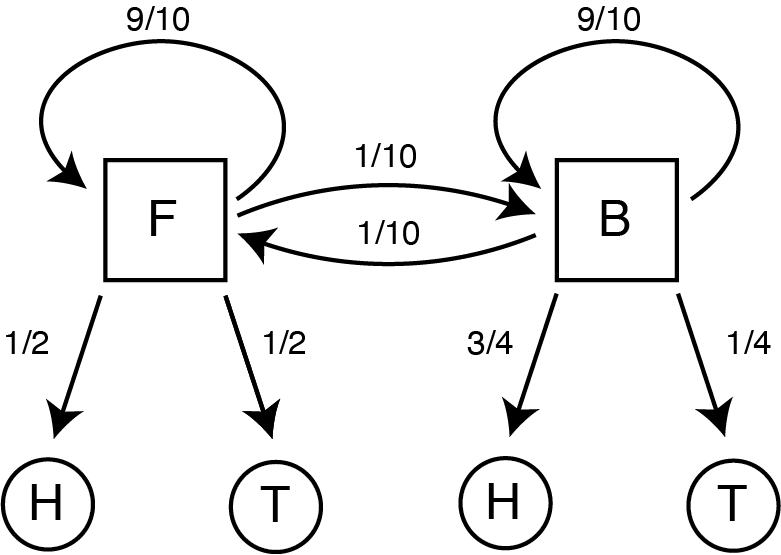
\includegraphics[scale=0.6]{../Figures/hmm_fair_casino.png}
			%	\end{subfigure}
	\end{figure}
\end{frame}

\begin{frame}{Hidden Markov Chains (Genomics)}
	Another (unrealistic) example is to build a HMM to describe a (genetic) sequence
	
	\begin{figure}[h]
	\centering
	%	\begin{subfigure}{0.4\textwidth}
		%		\centering
		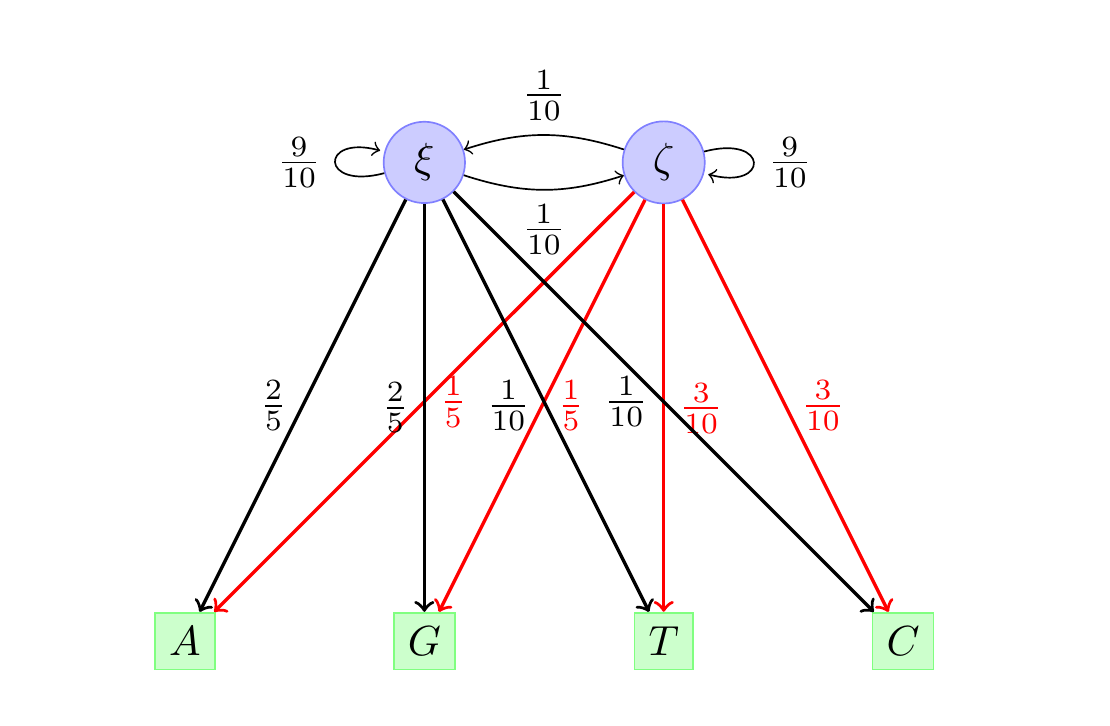
\includegraphics[scale=0.5]{../Figures/hmm_example.png}
		%	\end{subfigure}
\end{figure}
\end{frame}
\begin{frame}{Viterbi's representation HMMs}
		\begin{figure}[h]
		\centering
		%	\begin{subfigure}{0.4\textwidth}
			%		\centering
			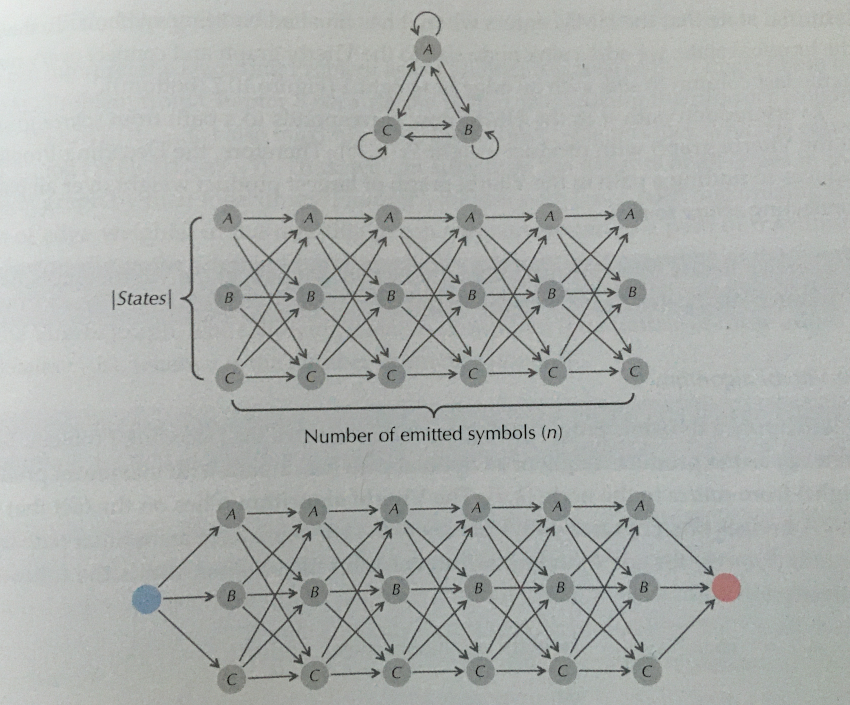
\includegraphics[scale=0.6]{../Figures/fig_hmm.png}
			%	\end{subfigure}
	\end{figure}
\end{frame}

\begin{frame}{Building a HMM}
	From Baker et al. 2014
\begin{quote}	
Here, we present a study that identifies transient networks of brain activity, with no prior assumptions
on the brain areas or time scales involved. This uses a distinct methodology based on a hidden
Markov model (HMM), which infers a number of discrete brain states that recur at different points in
time. Each inferred state corresponds to a unique pattern of whole-brain spontaneous activity, which
is modeled by a multivariate normal distribution and a state time course indicating the points in time
at which that state is active. These two outputs are shown schematically in Figure 1, and allow us to
describe both the spatial and temporal characteristics of each inferred state.
\end{quote}
\end{frame}

\begin{frame}{Building a HMM}
		\begin{figure}[h]
			\centering
			%	\begin{subfigure}{0.4\textwidth}
				%		\centering
				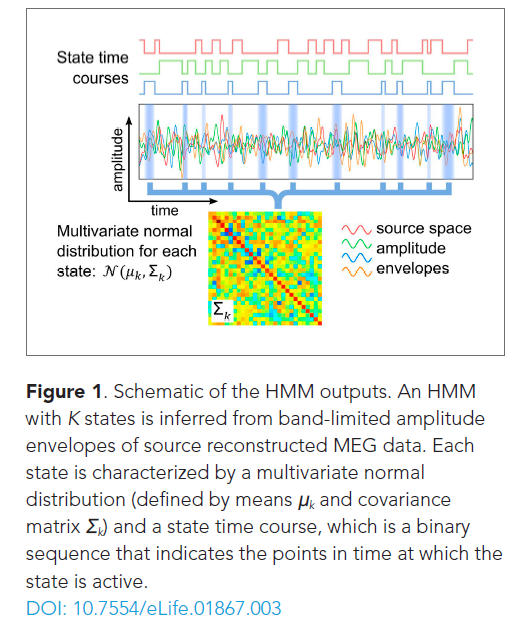
\includegraphics[scale=0.6]{../Figures/fig_hmm_baker.png}
				%	\end{subfigure}
		\end{figure}
\end{frame}

\begin{frame}{In the paper}
	
\begin{quote}
	The HMM is a family of models that can describe time series of data
	using a discrete number of states, all having the same probabilistic distributions
	but each having different distribution parameters. Thus, the
	states correspond to unique patterns of brain activity that recur in
	different parts of the time series. For each time point t, a state variable
	dictates the probability of each state being active at that moment
\end{quote}
\end{frame}

\begin{frame}{General HMM at rest}
			\begin{figure}[h]
		\centering
		%	\begin{subfigure}{0.4\textwidth}
			%		\centering
			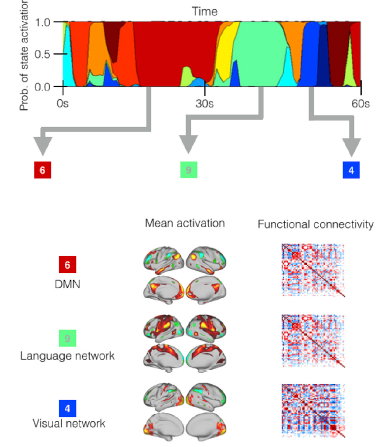
\includegraphics[scale=0.6]{../Figures/fig_vidaurre_1a.png}
			%	\end{subfigure}
	\end{figure}
\end{frame}

\begin{frame}{General HMM in task}
	\begin{figure}[h]
		\centering
		%	\begin{subfigure}{0.4\textwidth}
			%		\centering
			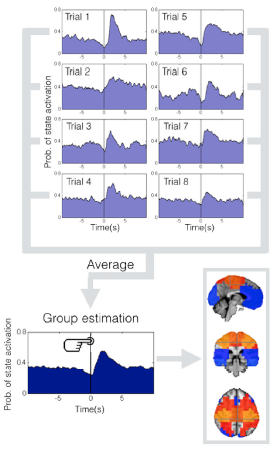
\includegraphics[scale=0.6]{../Figures/fig_vidaurre_1b.png}
			%	\end{subfigure}
	\end{figure}
\end{frame}

\begin{frame}{General HMM cont }
\begin{quote}
	an HMM
	generally comprises the description of the states, the state time courses
	(which determines the probability of each state to be active at each time
	point in the time series) and the transition probabilities between the
	states (i.e. the probability to transition from each state to each other
	state). Because here we run the HMM on all concatenated subjects'
	datasets, the states and the transition probabilities are defined at the
	group level; the state time courses are however particular to each subject
	- that is, states can come active at different moments for each subject.
	Since the probability distribution of each part of the model depends on all
	others, there is no closed-form solution available
\end{quote}
\end{frame}
%\begin{frame}{References}
%	Materials and some of the pictures are from \citep{calin}.
%	\printbibliography 	
	
%	I have used some of the graphs by hacking TiKz code from StakExchange, Inkscape for more aesthetic plots and other old tricks of \TeX
	
%\end{frame}


\end{document}
